\section{General UI Exploration}
\label{research:GeneralUIExploration}
\textbf{Source:} \cite{Juxtopposed}
A visually pleasing and easily operatable UI Is a core fundamental of my artifact and one I wanted to ensure I made correctly. As with other areas of research I started by casting a wide net across the internet to find resources I could study and learn from.

\subsection*{General:}
I cam across a YouTube Chanell named Juxtopposed which broke down User design ideals in a very clear and entertaining way - watching these videos soon became an enjoyable relaxation time for me whilst also letting me improve my EPQ, win win! Whilst all of her videos were highly informative I found the series redesigning large corporate Ui designs to be especially fascinating. 

Here she would break down preexisting UI layouts element be element whilst critiquing design decisions but also showcasing improved designs, the explanation following these changes was super informative to me, not just about producing aesthetically pleasing designs, but also making them accessible and intuitive 

\begin{figure}[H]
\centering

\includegraphics[width=0.8\textwidth]{Research/14_GeneralUIExploration/media/juxtaposed.png}
\caption{Juxtoposed YouTube Channel}
\end{figure}

\subsection*{Note-taking:}

\begin{figure}[H]
    \centering
    \begin{minipage}[t]{0.48\textwidth}
        \centering
        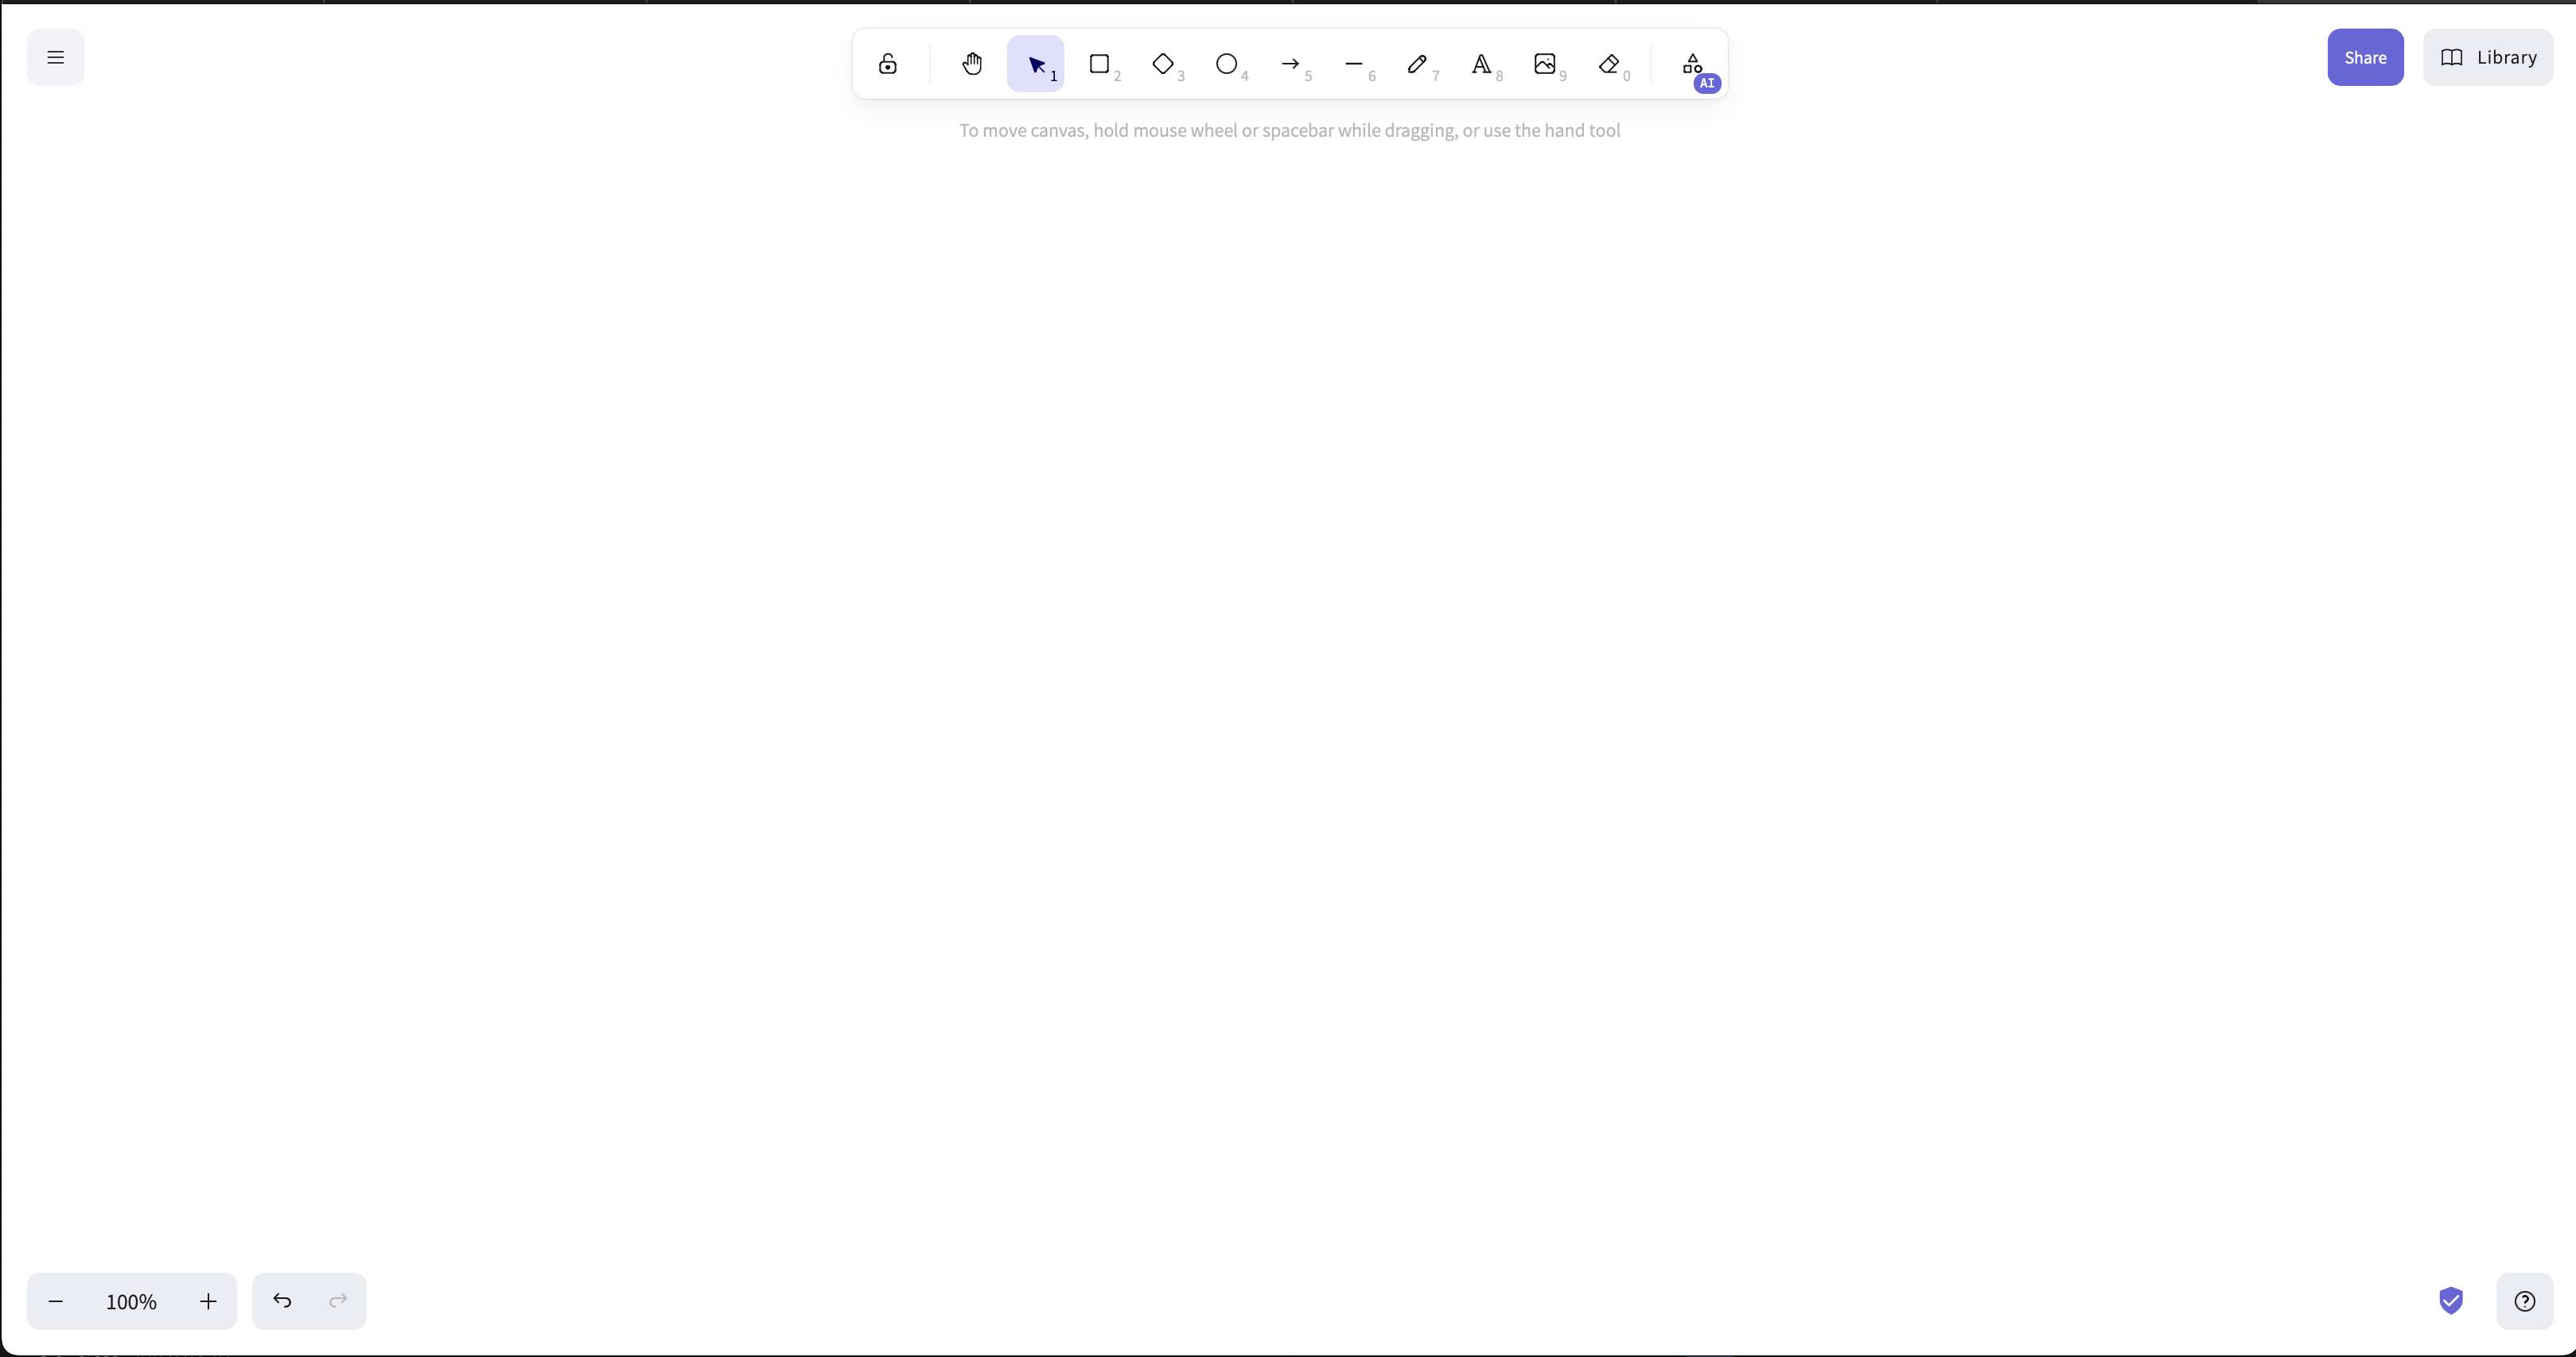
\includegraphics[width=\textwidth]{Research/14_GeneralUIExploration/media/excalidraw.png}
        \caption{Excalidraw Interface}
    \end{minipage}
    \hfill
    \begin{minipage}[t]{0.48\textwidth}
        \centering
        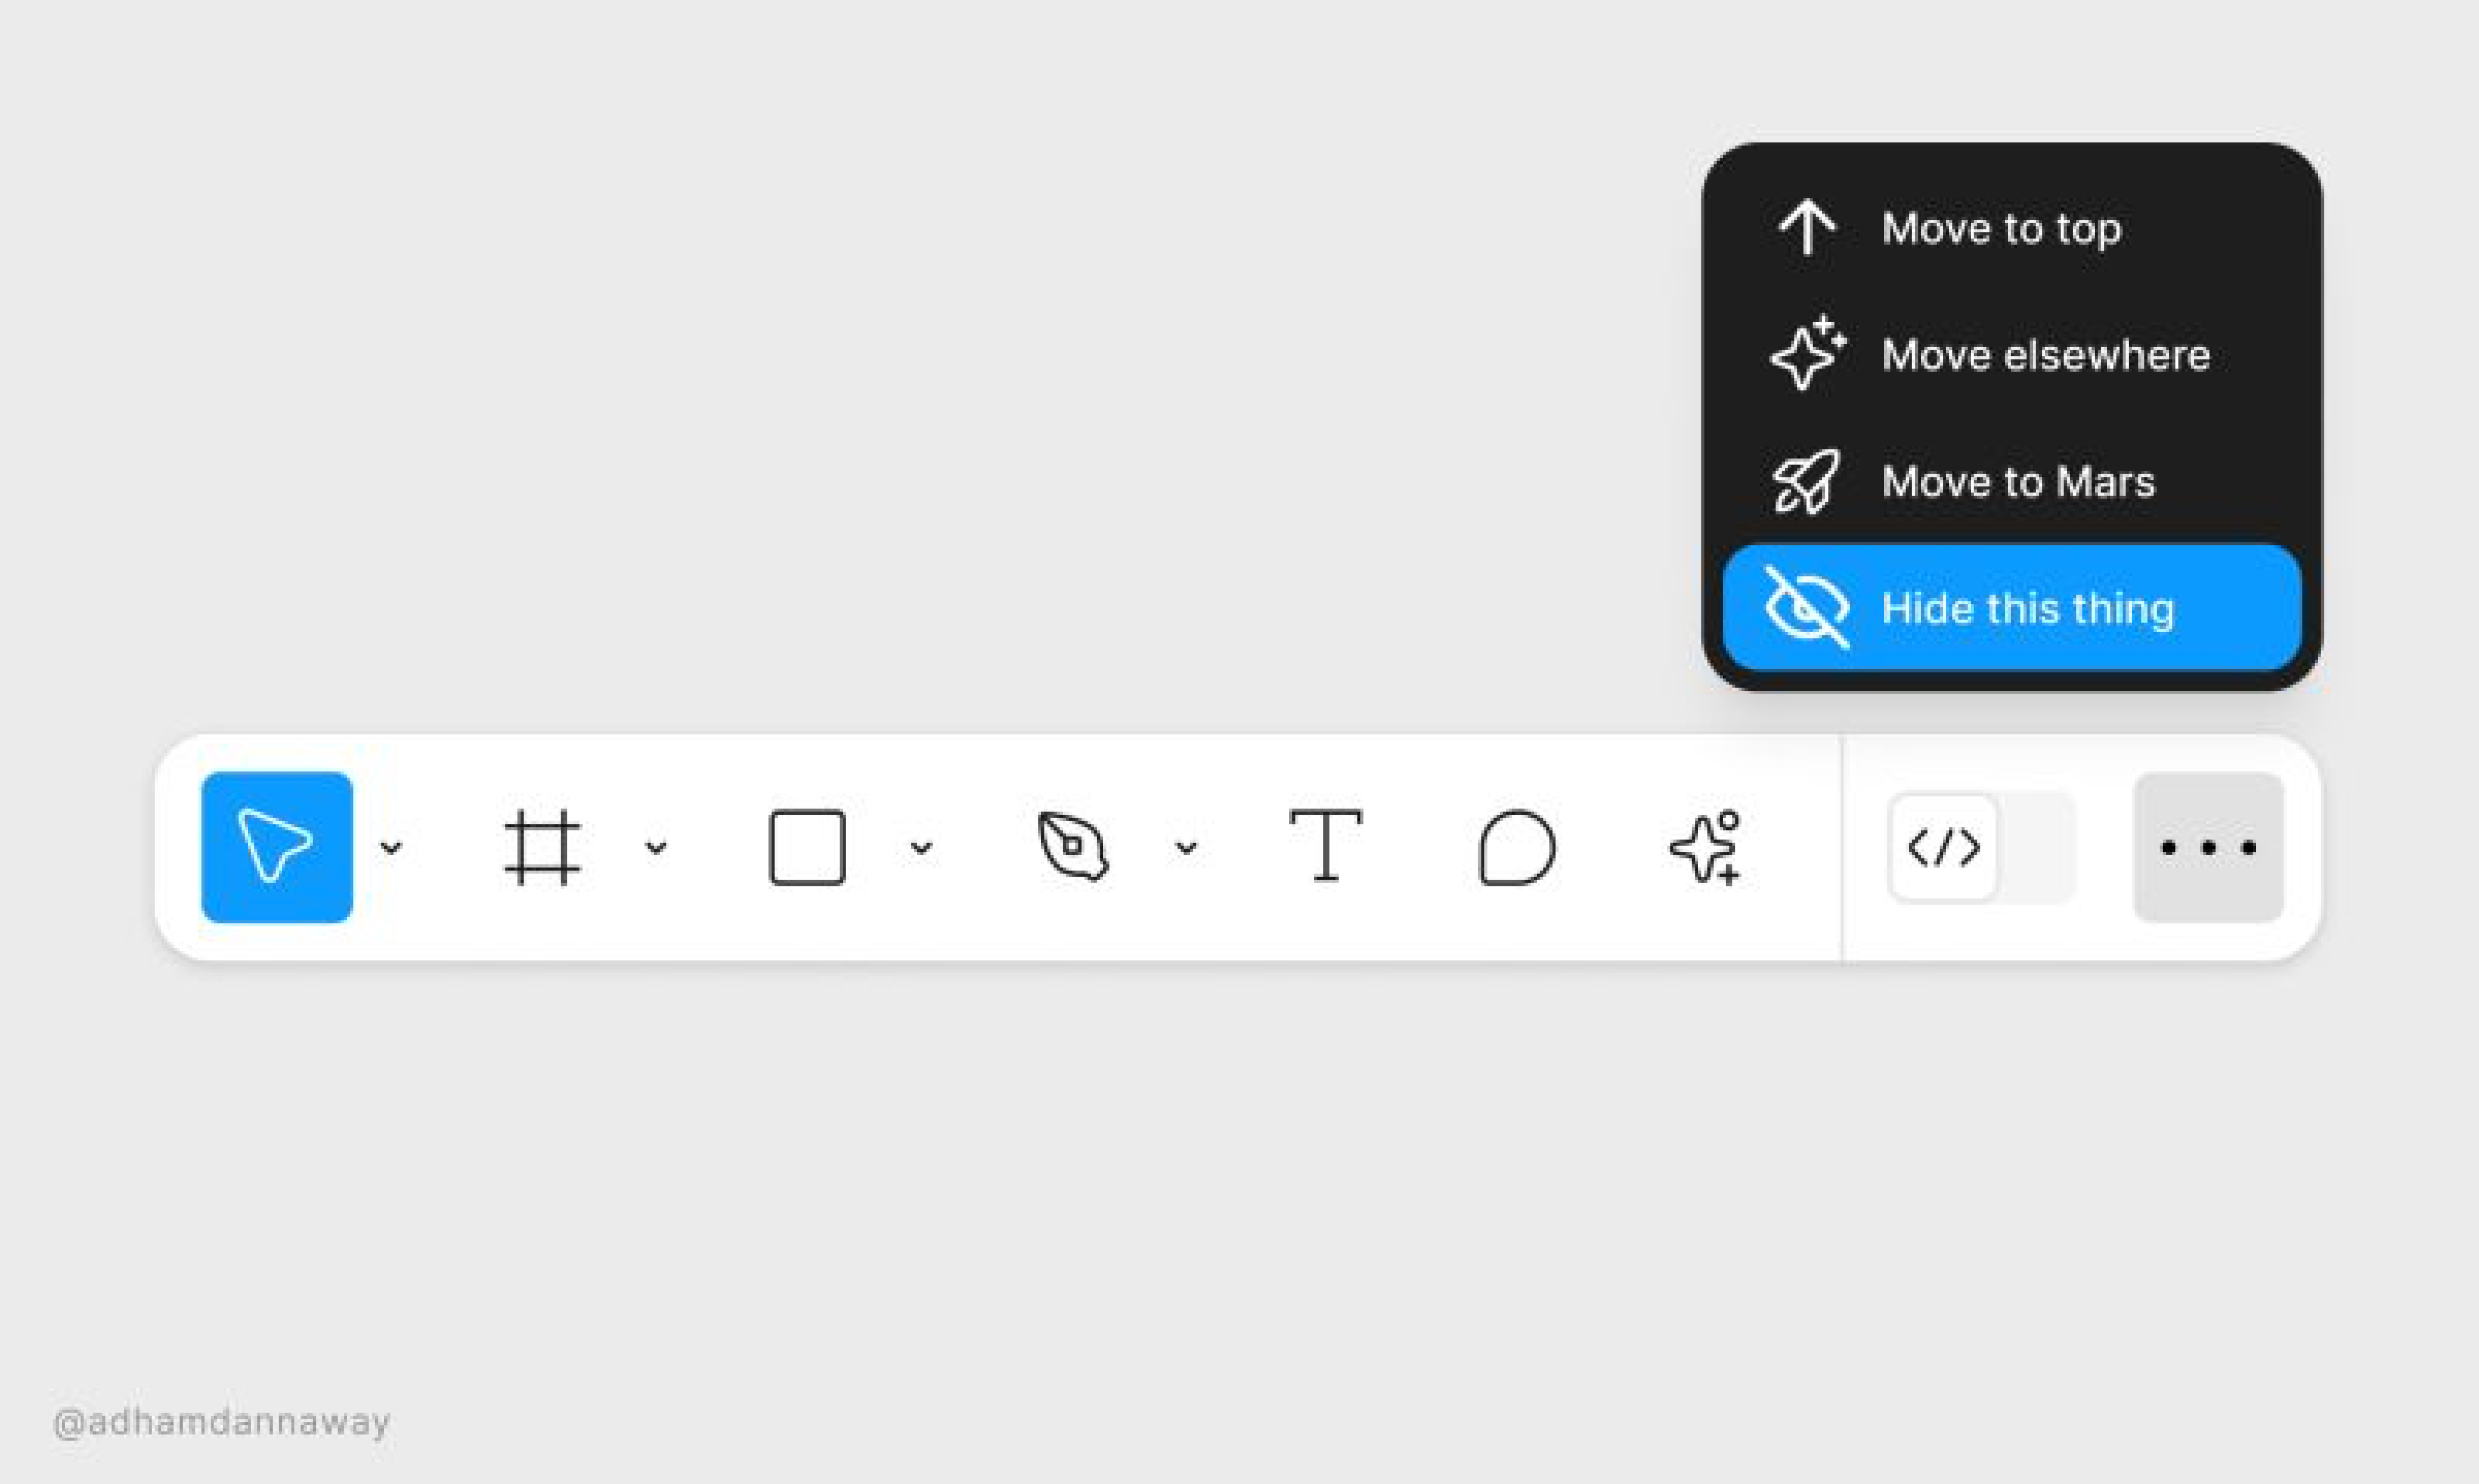
\includegraphics[width=\textwidth]{Research/14_GeneralUIExploration/media/figma.png}
        \caption{Figma Interface}
    \end{minipage}
\end{figure}

Both Excalidraw and Figma use 'floating' toolbars pinned to the top/bottom of the screen to display frequently used options to the user. These floating bars are accessible to both keyboard and mouse. Figma additionally places further options in a floating context menu if the dropdown next to a button is pressed


\subsection*{Dashboard:}

\begin{figure}[H]
    \centering
    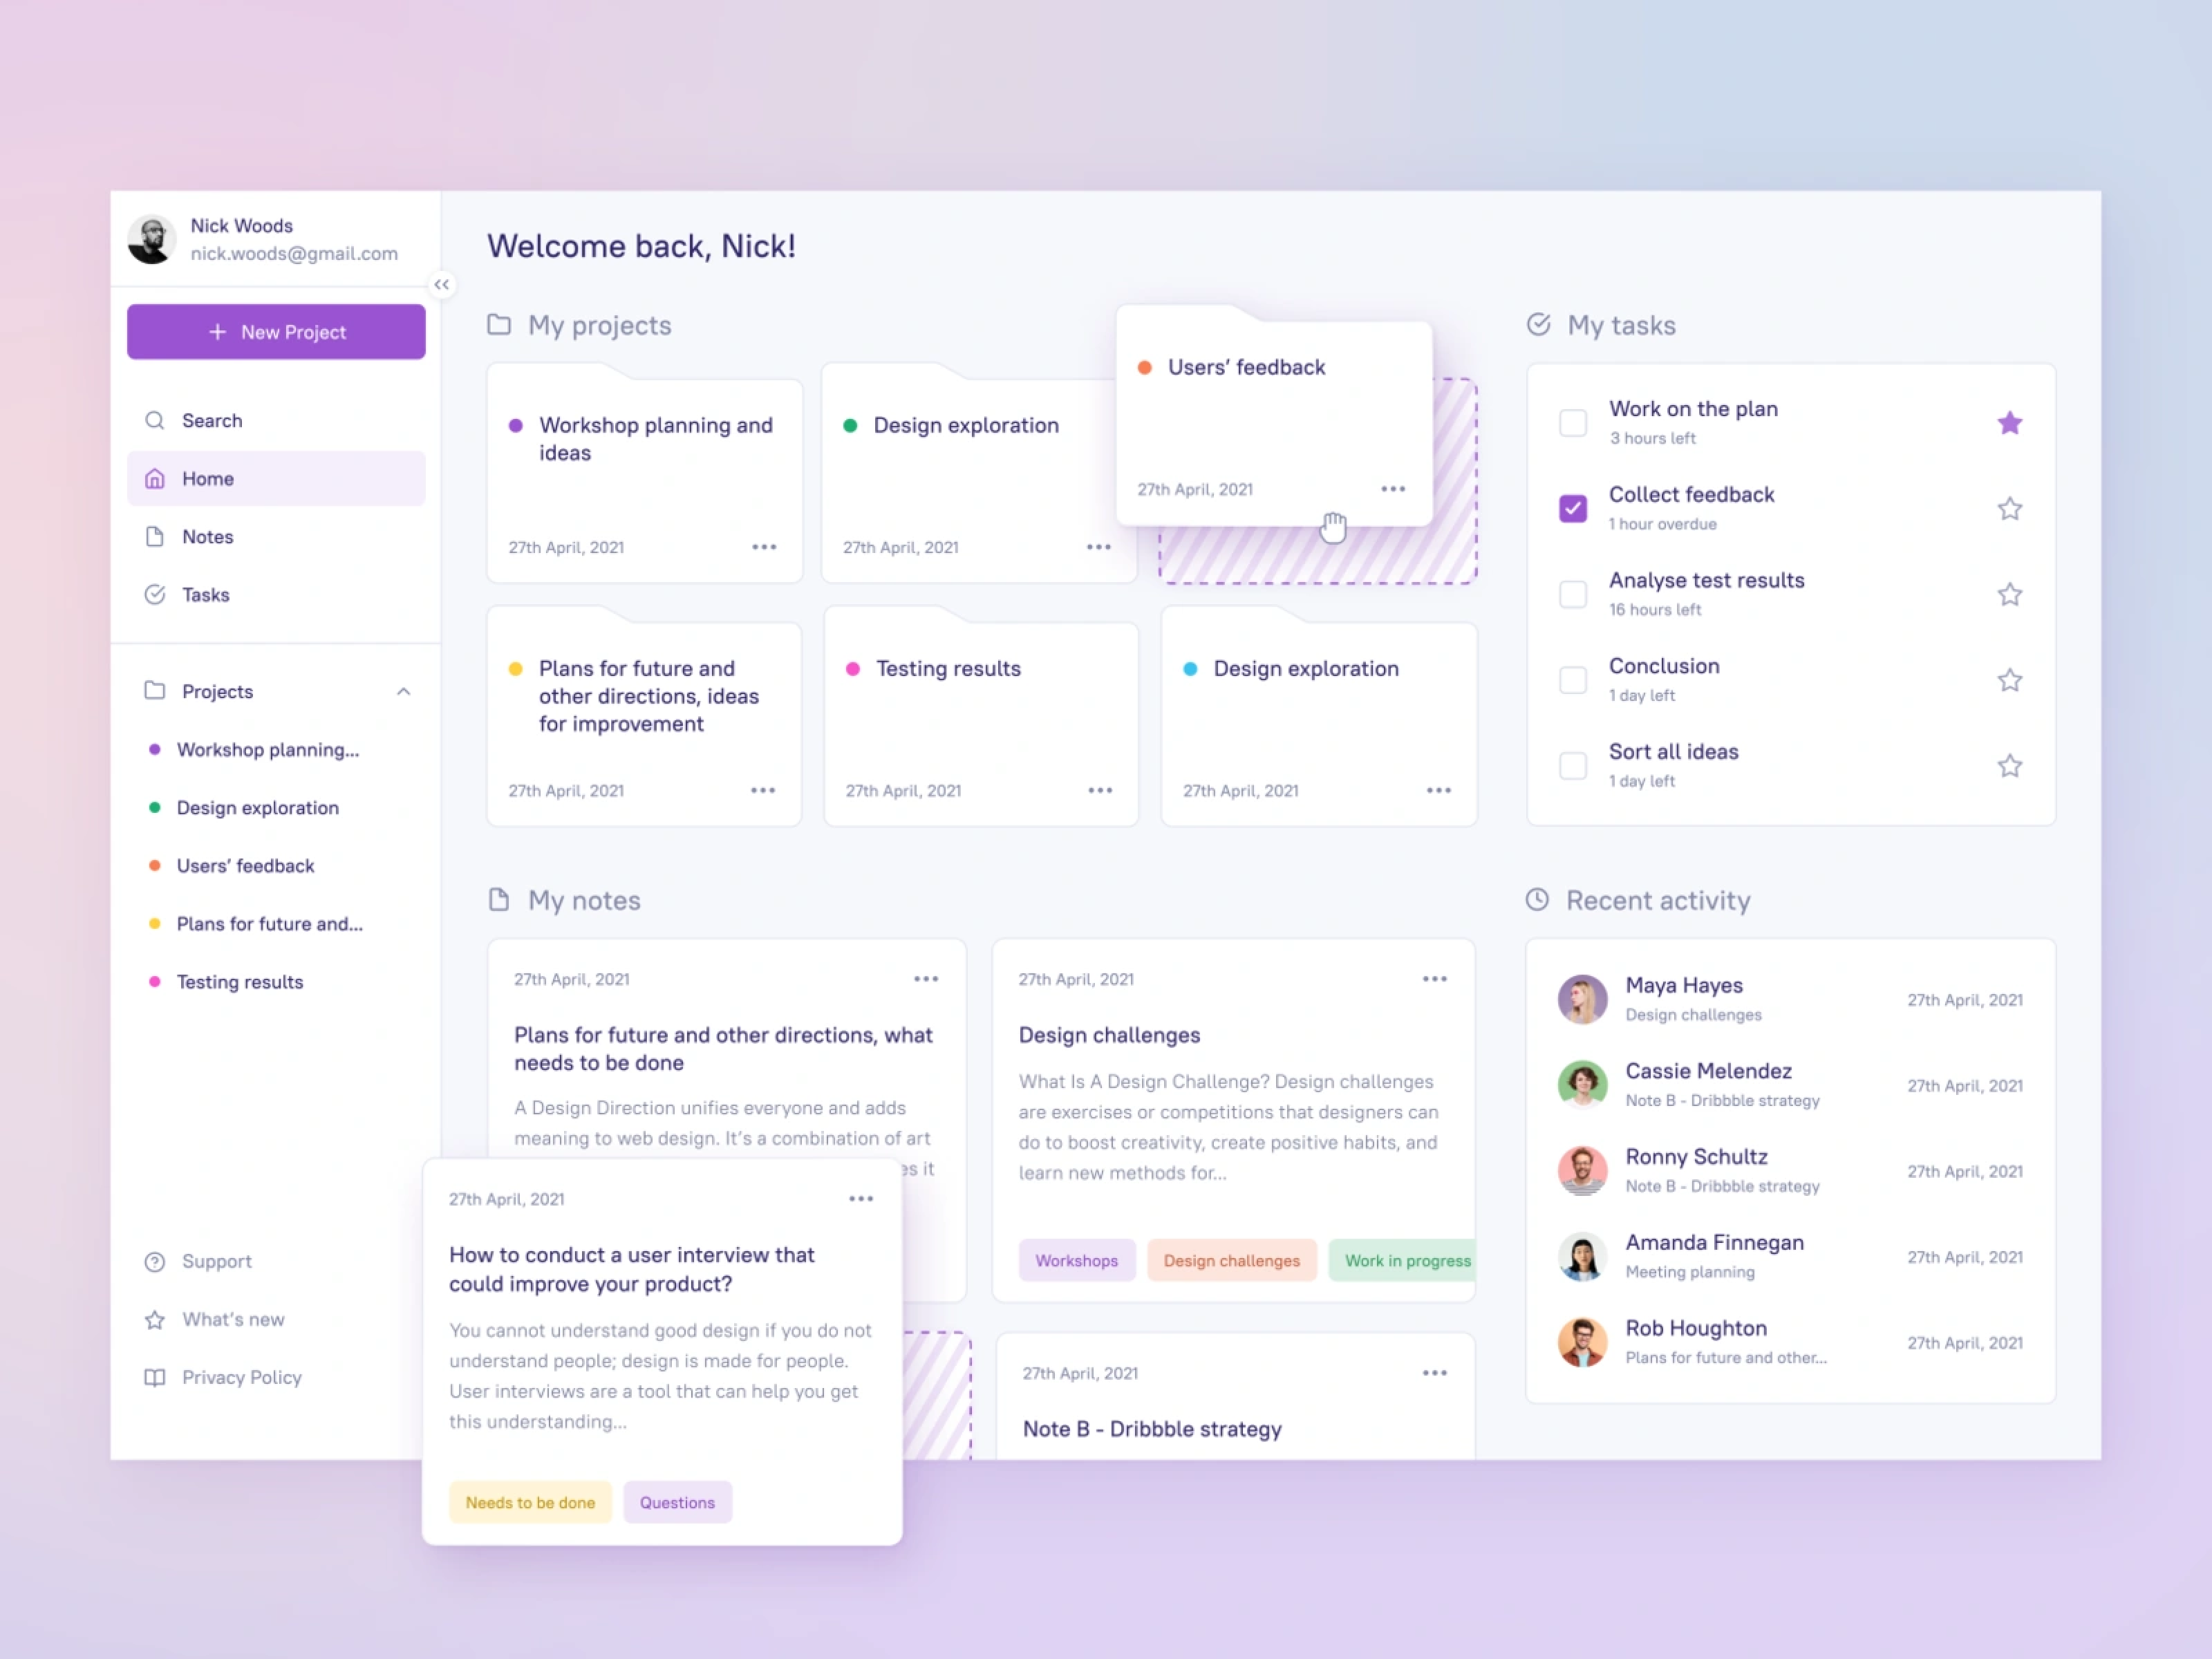
\includegraphics[width=0.8\textwidth]{Research/14_GeneralUIExploration/media/pastelDashboard.png}
    \caption{Pastel Dashboard}
\end{figure}
This dashboard design uses nice pastel colours, a core sidebar and separate compartments covering the main content.

The only downsides to this design is a lack of visual hierarchy which can make it hard to see which element is to be focused on

\begin{figure}[H]
    \centering
    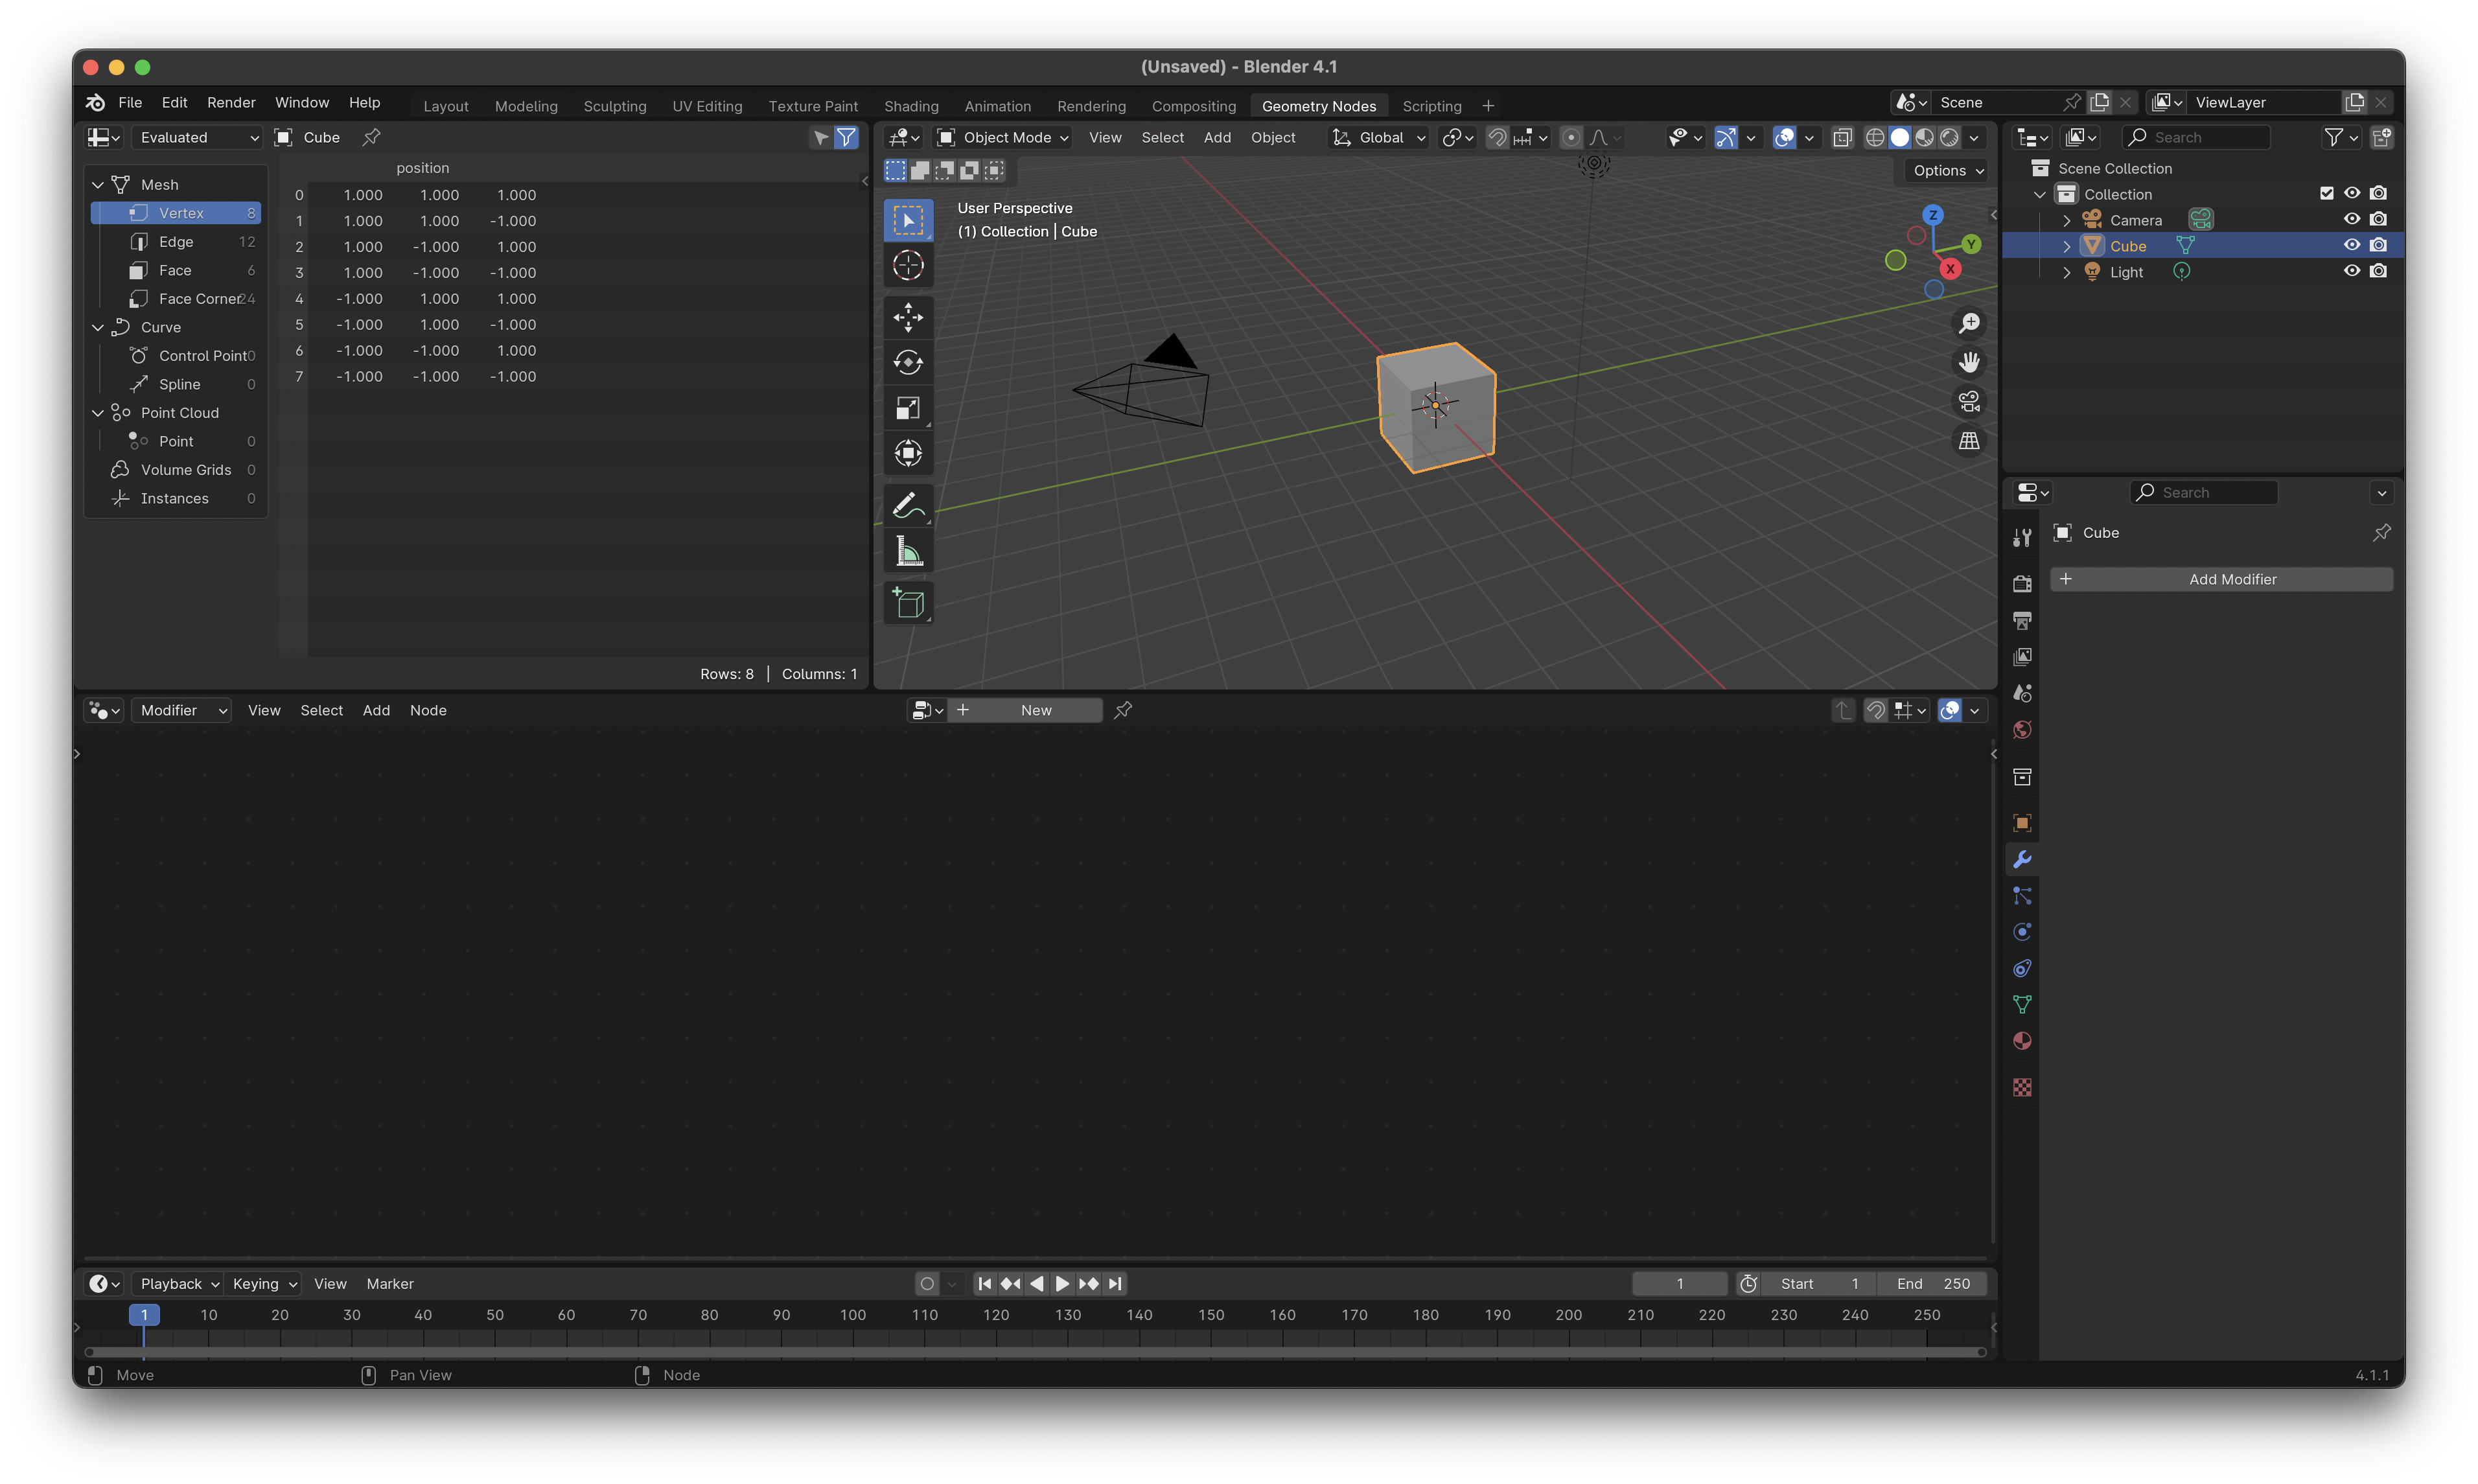
\includegraphics[width=0.8\textwidth]{Research/14_GeneralUIExploration/media/blender.png}
    \caption{Pastel Dashboard}
\end{figure}
This interface taken from the 3d modelling software blender is much more utilitarian in design but includes a very powerful and flexible panels view, for each 'panel' (the squares you see holding interface elements), you can change the type by clicking the top left button which opens a dropdown menu, new panels can be opened next to a current element by dragging and all panels can be resized. Whilst complicated this system allows fine tuning so that a user can see exactly what they want to see and any unnecessary information can be hidden

\subsection*{Login:}
\begin{figure}[H]
    \centering
    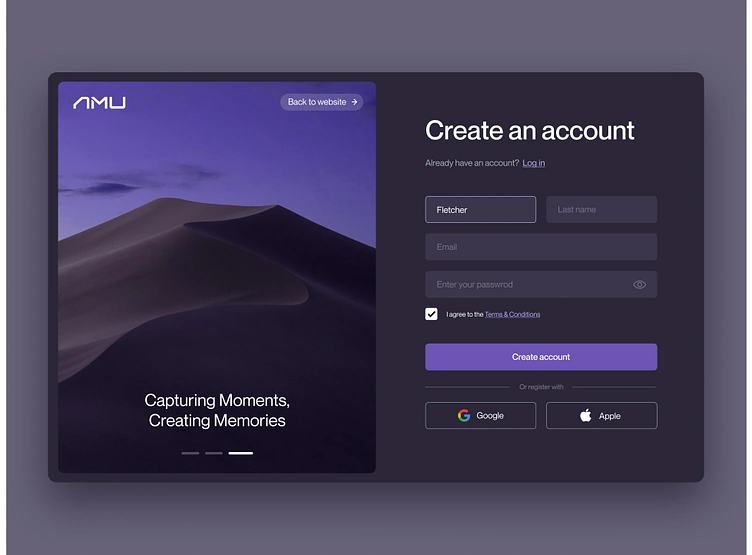
\includegraphics[width=0.8\textwidth]{Research/14_GeneralUIExploration/media/login.png}
    \caption{Login Interface}
\end{figure}
This design showcases a very visually appealing login screen that is perfect for larger screens. I really like the combination of imagery on the left and compact yet well organised input fields on the right. For mobile / smaller screens however this design would need to be reimagined to ensure better screen usage (most likely overlaying the input fields over a blurred version of the same images) 

\subsection*{Vertical tabs:}
\begin{figure}[H]
    \centering
    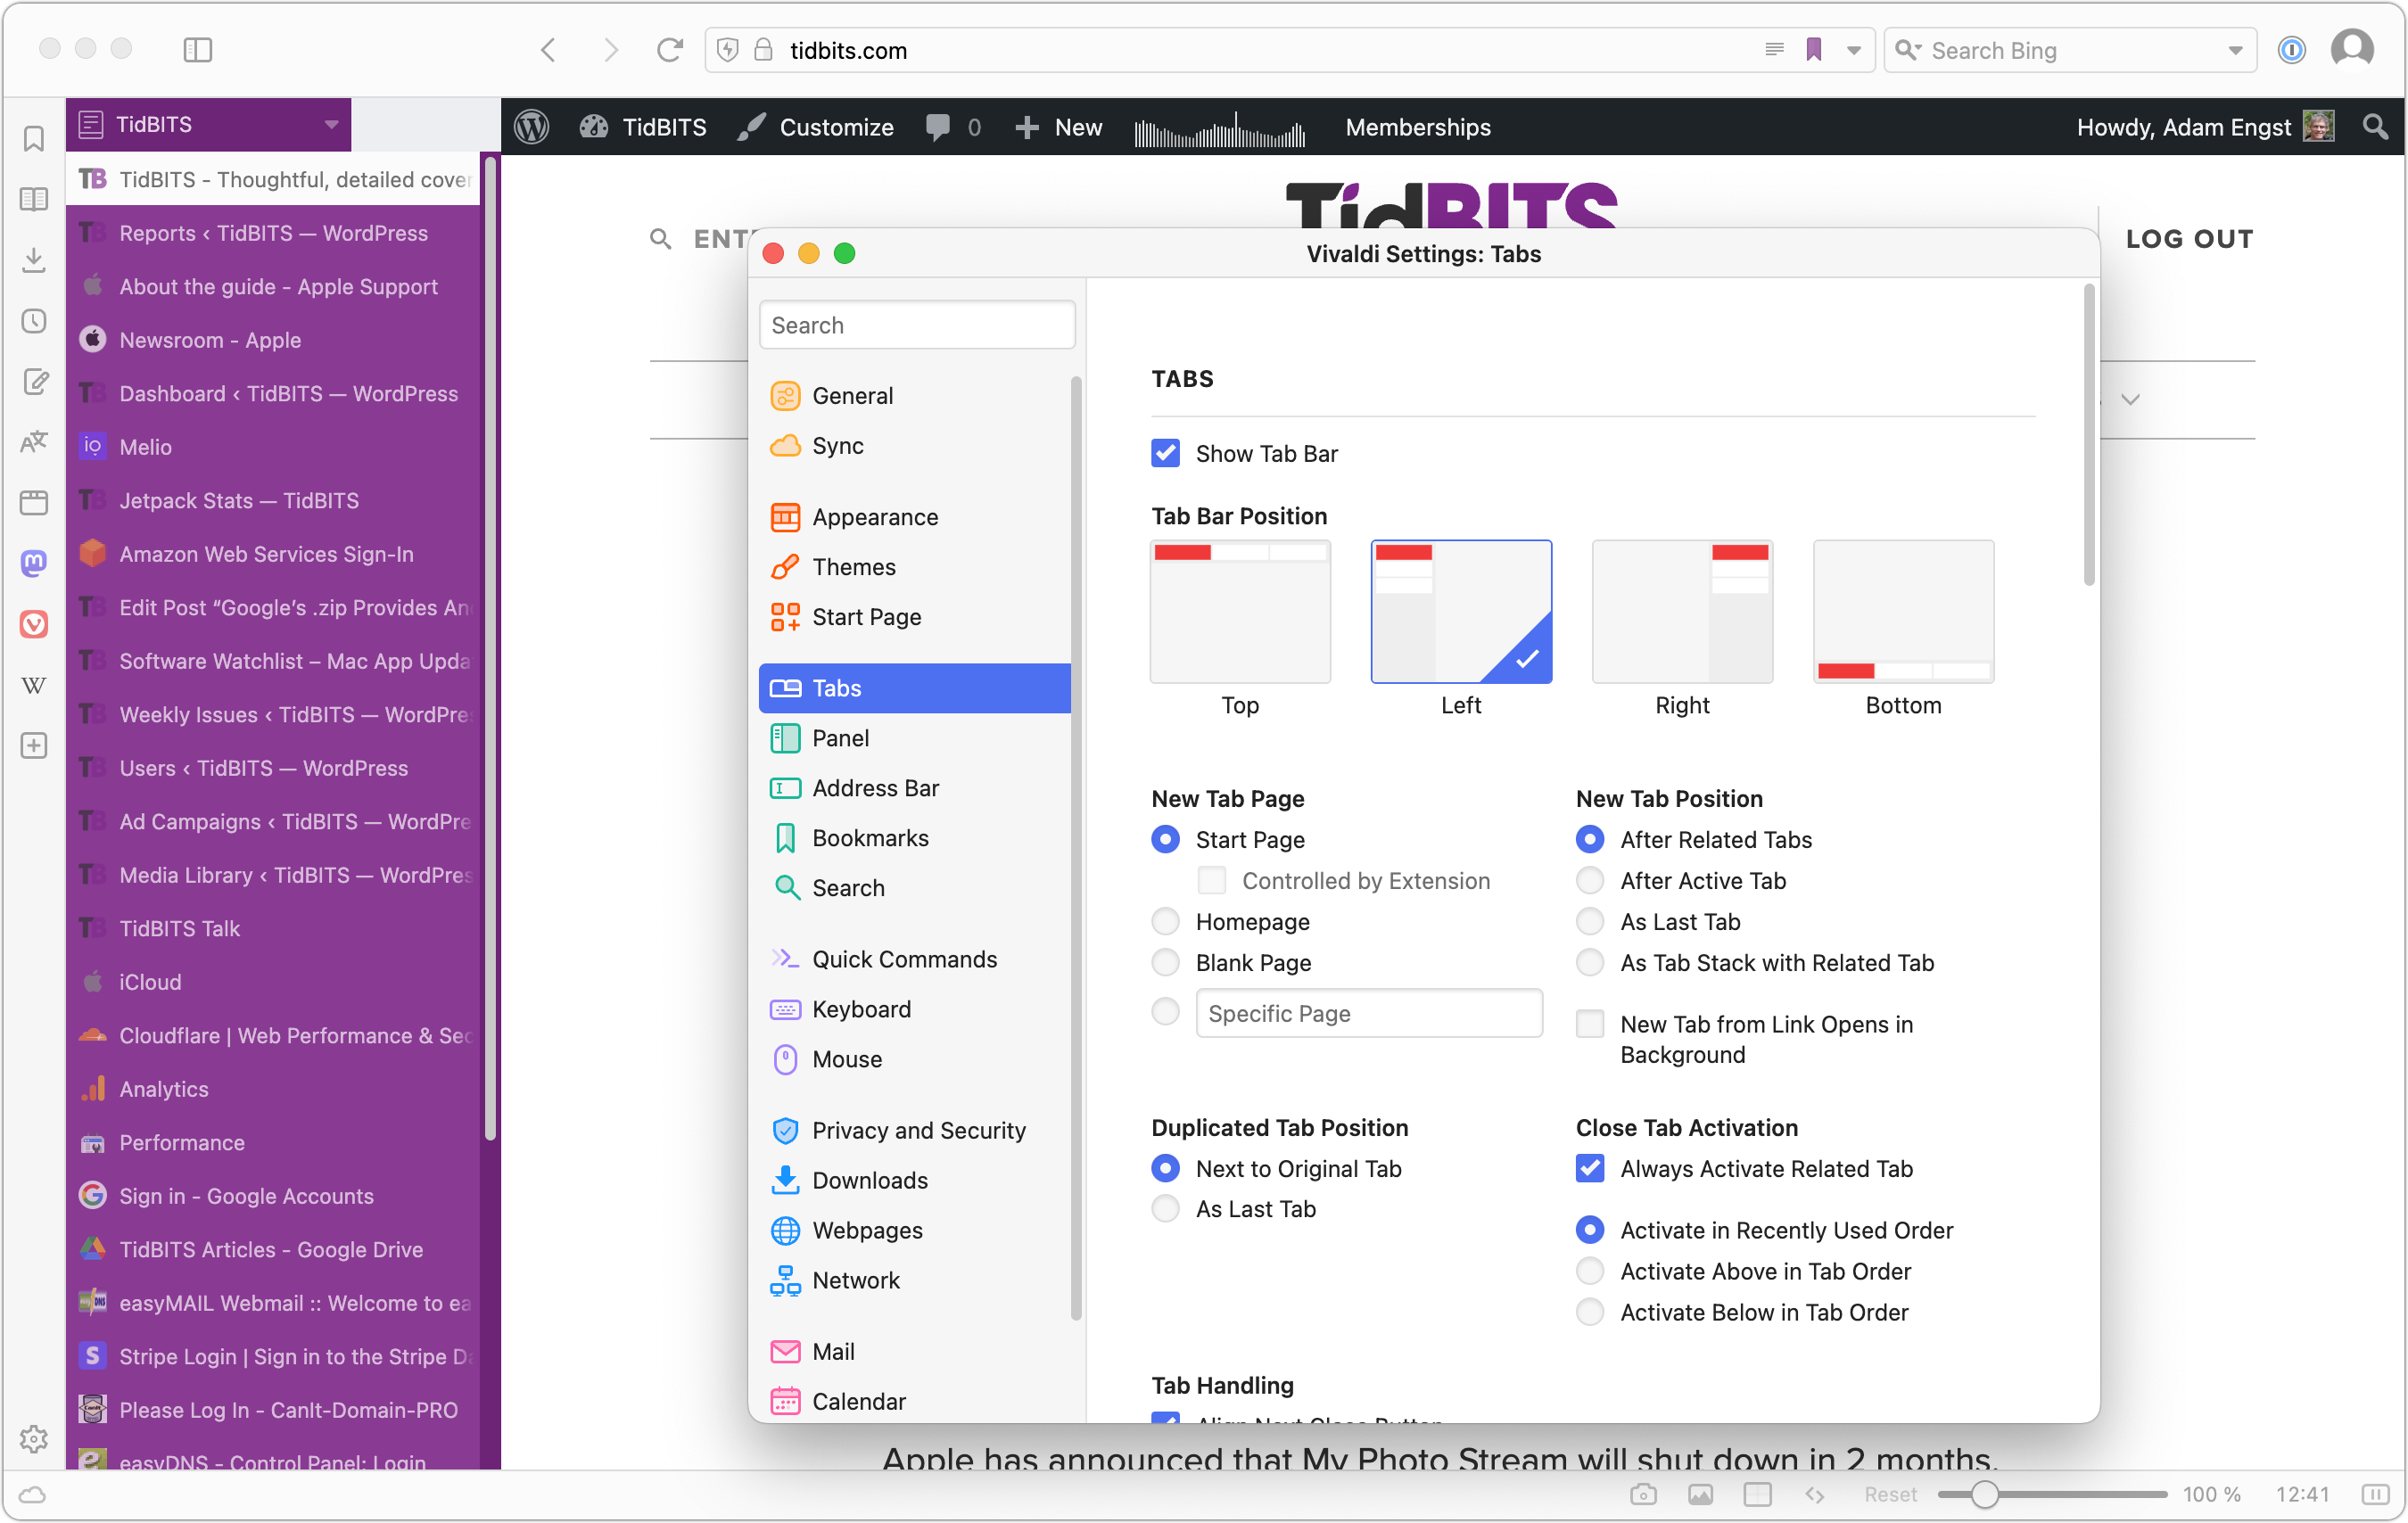
\includegraphics[width=0.8\textwidth]{Research/14_GeneralUIExploration/media/verticalTabs.png}
    \caption{Vertical Tabs}
\end{figure}

Vertical tabs are used by many applications to give users an organised breakdown of each open 'session'. Compared to horizontal tabs, vertical tabs are much more space efficient and are able to more easily fit options such as tab pinning and closing


